\section{Methodology}
\label{sec:method}

We propose the tool workflow illustrated in Figure~\ref{fig:workflow} for
studying software evolution via VCS data. First, each version of all source
files in the project are reconstituted from the differences stored within the
VCS such that each version of a file can be parsed by an appropriate language
front end.  Each front-end is configured to map the parsed code to an aterm
that represents a standardized serialization of the AST\@.  Mapping languages
to a common aterm format allows the downstream portions of our workflow to be
language-agnostic to a large degree, with minimal language-specific
parameterization.

\begin{figure}
\begin{center}
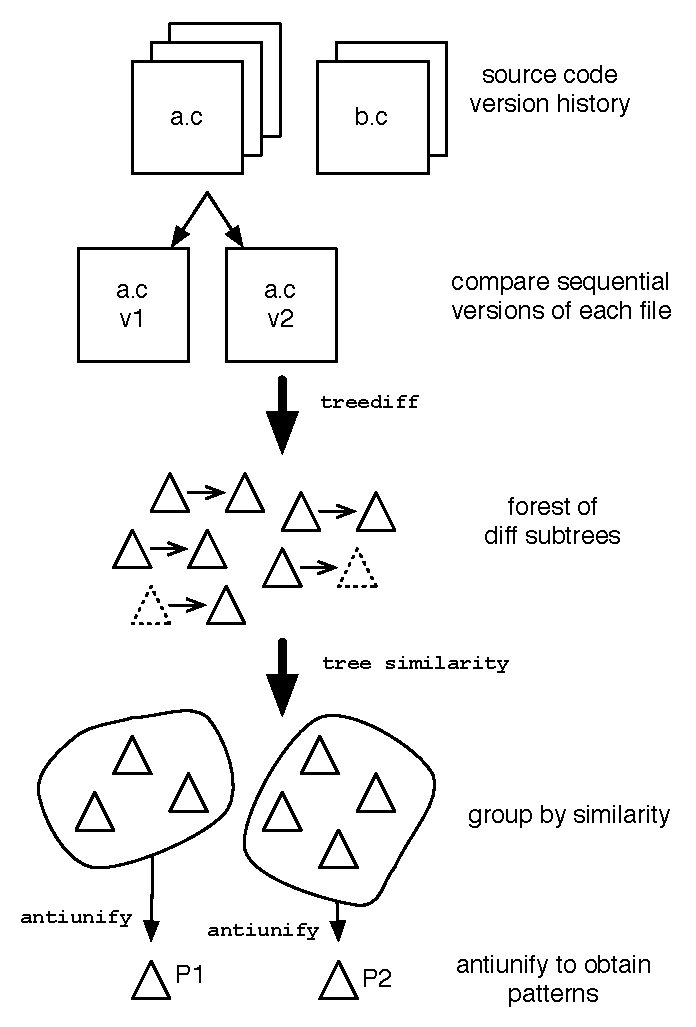
\includegraphics[height=0.44\textheight]{figures/workflow.pdf}
\caption{The components of our prototype indicating how VCS data is
broken down into groupings of related changes for pattern generation.}
\label{fig:workflow}
\end{center}
\end{figure}

Once we have code in an aterm format, we can then apply a structural
differencing algorithm between adjacent versions of each source file (e.g.,
version $n$ of file $f$ is compared to version $n+1$ of file $f$).  The result
of this is a forest of trees that represent the portions of the AST of file
$f$ that changed between versions at the structural level.  These changes can
either be code insertions, deletions, or mutations.  Our differencing is based
on the work of Yang~\cite{yang91diff} whose algorithm was designed for
computing differences between source code versions.  Yang's goal was to
improve the visual presentation of differences in textual diff tools, and our
use of their algorithm to provide input to further tree analysis algorithms is
novel.

After reducing the sequence of differences stored in the VCS, we have a large
forest of trees each representing a change that occurred over the evolution of
the software.  At this point, we seek to relate each of these trees via a
tree similarity metric.  This is achieved by using Yang's algorithm a second
time, but in this case we ignore the sequence of edit operations that it
produces and simply consume the quantitative similarity metric that it
produces as a rough estimate of how closely related two trees are.  A
threshold parameter is defined in which two trees with a similarity above the
threshold are considered to be part of the same group of difference tress.

Finally, once the set of differences are grouped into groups of trees that are
similar up to the threshold, we perform antiunification on the entire group to
distill all members to a representative code pattern for the group.
Antiunification of a set of terms yields the least general generalization of
those terms, which is how we define our notion of a code pattern.  The
antiunification algorithm as described by Bulychev~\cite{bulychev08dupe} as
part of the {\it clonedigger}
project\footnote{\url{http://clonedigger.sourceforge.net}} was used, which
itself is an implementation of the classical antiunification algorithm
described by both Reynolds~\cite{reynolds70antiunification} and
Plotkin~\cite{plotkin70antiunification}.

In the following sections, we describe the steps above in greater detail.

\subsection{Parsing and aterm generation}

One of the most challenging aspects of performing this kind of study on
arbitrary software packages is the availability of robust language parsing
tools.  In the absence of a common intermediate representation or abstract
syntax representation for popular languages, we adopted a standardized
serialization format in the form of annotated terms.  Generation of aterms was
achieved via language-specific parsers.  In this work, we used the
{\tt language-java} parser available as an open source library accessible via the
Haskell programming language.

The structure of aterms is given by this simple syntax:
\setlength{\grammarindent}{8em}
\begin{grammar}
<aterm> ::= `AAppl' <string> <aterm-list>
\alt `AList' <aterm-list>
\alt `AInt' <int>

<aterm-list> ::= <aterm> <aterm-list>
\alt $\epsilon$
\end{grammar}

This structure is sufficient for us to encode typical abstract syntax trees if
we allow ourselves to use the string label of the {\tt AAppl} portion of the
aterm. This is most easily illustrated with an example.  Suppose that we have
the Java AST for the statement {\tt i++;}.  In a textual form, this portion of
the AST would be represented by:

\begin{verbatim}
ExpStmt
  (PostIncrement
    (ExpName
      (Name [Ident "i"])))
\end{verbatim}

The translation to aterm would give us:

\begin{verbatim}
AAppl "ExpStmt"
  [AAppl "PostIncrement"
    [AAppl "ExpName"
      [AAppl "Name"
        [AAppl "Ident" [Appl "\"i\"" []]]]]]
\end{verbatim}

Notice that for strings, such as identifier names, we place double quotes
around the string inside the label portion of the aterm. Implementations of
aterms often provide a representation that allows for nodes to be shared
within the tree. While this is a useful optimization for saving space, we
chose to use the simpler unshared representation in our prototype due to the
clearer expression of the tree analysis algorithms over the unshared form of
the structure.

\subsection{Structural differencing}

One of the classical algorithms studied in computer science is that of string
similarity and the concept of string edit distance as a measure of the minimal
number of operations necessary to mutate one string or sequence into another.
A more complex problem is to define a similar sequence of operations to change
a non-linear structure like a tree from one into another.  This problem of
computing a structural edit distance has been studied since the 1970s and has
yielded tree differencing algorithms analogous to string differencing
algorithms commonly used in text analysis.  Many modern efforts in this area
are based on the initial work of Selkow~\cite{selkow77tree} and
Tai~\cite{tai79tree}.  Interest in such analysis of tree-structured data
increased with the proliferation of structured document formats used on the
Internet such as XML, HTML and SGML (a noteworthy example from this body
of work is found in Chawathe~\cite{chawathe96change}).

Our work is based on Yang's source differencing technique~\cite{yang91diff}.
In this algorithm two trees to be compared are mapped to two trees of edit
operations in which nodes from the original trees are annotated with edit
operations ({\it keep} or {\it delete}).  These can be applied to turn each tree into the
other.  On their own the edit trees are not sufficient to identify the paired
subtrees that represent regions where change occurred.  This requires an
additional step of processing the edit trees to form a single tree in which the
edit trees have been woven together.

\subsection{Identifying structural changes via edit tree weaving} 
\label{sec:weaving}

Ideally, we would like to obtain from the tree differencing algorithm what can
be thought of as the two trees overlaid on each other such that the common
structure from the root towards the children is clear, and points where subtrees
differ are explicitly identified.  The details on how this algorithm was 
implemented are not critical to this paper --- instead, we will focus on what the
woven trees contain.  In the discussion that follows, we adopt the 
convention that the arguments to the binary tree differencing function are
referred to as the \emph{left} and \emph{right} trees.  

Changes that occur between the trees are represented by three change types. If
the difference between two trees is the insertion of a subtree in the right
tree, then the woven tree will contain a \emph{left-hole}.  Similarly,
deletion of a subtree from the left such that it is not present in the right
tree will result in a \emph{right-hole}.  If a subtree was determined to be
changed, then the woven tree will contain a \emph{mismatch} point that refers
to the both the right and left subtrees that differ.  All other points in the
tree that match are joined with a \emph{match} point that contains the
corresponding common node to both trees.  

% To separate the modifications into the different kinds, we consider the type of
% mismatch between the input trees. We refer to the tree before the change as the
% left tree and the tree after the change as the right tree. The weave tree joins
% together the parts of the tree that did not change and has special branches for
% the parts that are different. These special branches come in several varieties:
% left and right mismatches and left and right holes. We will often group left
% and right mismatches into simple mismatches.

% Left and right mismatches represent an edit to an existing node of the AST\@.
% A left mismatch represents the change before the edit and the right mismatch
% contains the change after the edit.  Using our previous example of the Java
% statement {\tt i++;}, if we changed this to {\tt j++;}, we could get a left
% and right mismatch where the left mismatch is {\tt AAppl
% "\textbackslash"i\textbackslash"" []} and the right mismatch is {\tt AAppl
% "\textbackslash"j\textbackslash"" []}. 

% A left hole represents the case where the left tree (before the edit) had nodes
% that are missing in the right tree (removed by the edit). A right hole is for
% the swapped case, where the left tree is missing nodes that are present in the
% right tree. Therefore, left and right holes represent an edit that removes or
% adds code respectively.

Given two edit trees that have been woven together into a tree with explicit
holes and mismatches, we can extract the subtrees that correspond to the three
types of changes above.  Match points also play an important role in
extracting changes by retaining the common context that was present in both
trees where the change occurred.  If we extract only the subtree rooted at the
point where the change occurred, the rest of the analysis will be missing the
context where the change took place. This information is necessary when
constructing understandable patterns.  

For example, while it may be true that a code fragment such as {\tt i++} is
where the change occurred, it is most useful to know whether or not that
fragment occurred within an expression, a for-loop, or as a standalone
statement. As such, we have chosen for the work presented here to extract the
subtree along with the closest enclosing statement. For example, if the
subtree was the expression {\tt i++;} within the statement {\tt if(i < 100)
i++;} we would extract the if-statement with the expression.

This is achieved by including the subtree rooted at the nearest ancestor
(which must be a matching point in the woven edit trees) to a change
representing an appropriate abstract syntax element.   In the future, we would
like to explore other ways of extracting context, such as looking at the
closest enclosing expression, function (when it exists), or class.  This
information should also be parameterizable to support differences in important
AST nodes that varies between languages.

\subsection{Tree similarity metric and grouping}

Given two trees $t_1$ and $t_2$, we would like to define a similarity metric
such that $d(t_1, t_2) \in [0,1]$, where a similarity of $1$ means that the
trees are identical, and $0$ represents maximal dissimilarity.  In Yang's
algorithm, a similarity score is provided for comparing $t_a$ and $t_b$. This
metric is order dependent, forcing the maximal score to be the size of the
left tree ($t_a$), even if $t_b$ is larger.  If the trees are identical, the
score will be exactly $|t_a|$, the number of nodes in $t_a$.  If they differ,
it will be strictly less than $|t_a|$.  As such, it would be possible to define
our distance function to be $\frac{d(t_a, t_b)}{|t_a|}$, but this operator is
not symmetric, since it is easy to find instances such that $\frac{d(t_b,
t_a)}{|t_b|} \neq \frac{d(t_a, t_b)}{|t_a|}$ when the trees are very different.
Instead, we define $\Delta(t_a, t_b)$ to be the function
$$\Delta(t_a, t_b) := \frac{min(d(t_a, t_b),d(t_b, t_a))}{max(|t_a|,|t_b|)}$$
where the $min$ and $max$ functions force the calculation to be symmetric.

Once we have the set of changes that were detected from the VCS history, we
can generate a forest of trees $t_1, \cdots, t_n$ obtained from the holes and
mismatch points in the woven edit trees.  We then compute the $n^2$ distances
between all pairs to generate a distance matrix $D$ where $D_{ij} =
\Delta(t_i, t_j)$.  Given a threshold value $\tau$, we can produce a boolean
matrix $D'$ where $D'_{ij} = \Delta(t_i, t_j) > \tau$.  An example matrix is
shown in Figure~\ref{fig:boolmat} for changes observed in the VCS for ANTLR
where $\tau = 0.9$.  Note that for large numbers of changes, a sparse
representation of the boolean matrix can be computed for a given $\tau$
without requiring the full dense distance matrix to be created.  The sparsity
of the matrix is dependent both on the types of changes present and the value
of $\tau$ chosen.  

\begin{figure}
\begin{center}
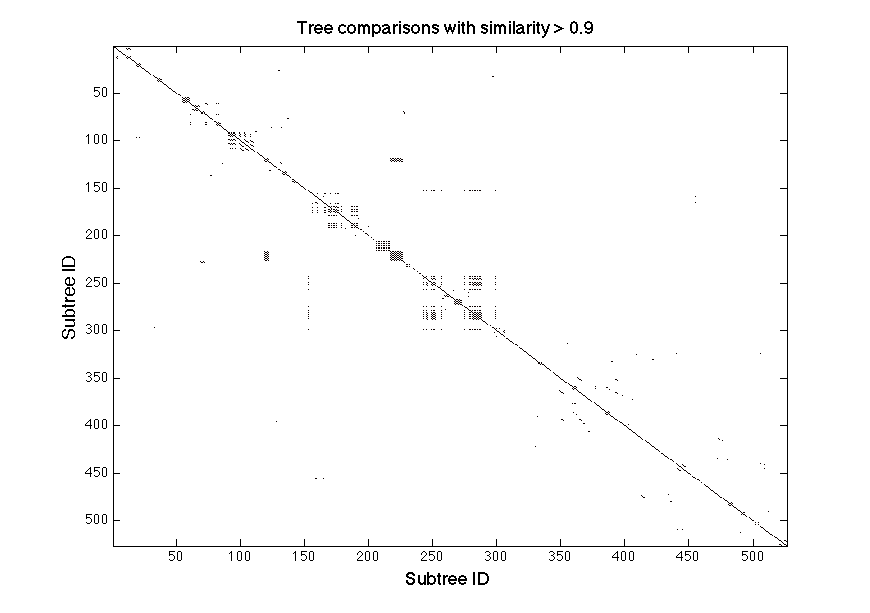
\includegraphics[width=0.45\textwidth]{figures/distmatrix-0-9.png}
\caption{Boolean matrix $D$ for over 500 changes from the ANTLR repository indicating all pairs of
changes for $\tau = 0.9$.}
\label{fig:boolmat}
\end{center}
\end{figure}

In our implementation, we create multiple distance matrices such that each
represents only related changes of a certain type from the woven tree (left
and right holes, and mismatches).  The matrix as defined above is simply the
element-wise boolean or of these three matrices.  Capturing this information is
important as it allows us to further refine our view of the code evolution to
distinguish code changes from the insertion or removal of code that occurs
over time. For example, when code is being developed and grown, we expect to
see a number of code insertions. Similarly, when a mass refactoring occurs to
simplify code, we would expect to see a set of code deletions.  When a more
subtle refinement occurs, such as transposition of code arguments or the
addition of a conditional to refine control flow, we would expect to see
mismatches where the tree changes.

%%% sparsity mentioned above
%\jason{Point out that even though this matrix is very sparse (and that's a
%problem for most data mining for changes in VCS history, our approach handles
%this like a champ and zooms in on the relevant bits.}

\subsection{Antiunification and template generation}

Once we have groups of related code snippets in the form of related subtrees,
we can seek patterns that relate changes.  For example, say we have a function
call {\tt foo()} where each invocation of the function uses the same
parameters (e.g, {\tt foo(x,y)}, where {\tt x} and {\tt y} are always the
same). If we add a new parameter at the end of each call where the variable
passed in differs each time (e.g., {\tt foo(x,y,a)} and {\tt foo(x,y,b)}), we
would like to abstract out this change as {\tt foo(x,y,\metavar)}, where each
instance of the change replaces \metavar~with whatever concrete variable is
used at that point. The antiunification algorithm is built for this purpose --
given two trees, it seeks the least-general generalization of the pair and
produces a triplet representing the generalized tree with a metavariable
introduced where the two differ, as well as a substitution set that allows the
metavariable to be replaced with the appropriate concrete subtree necessary to
reconstitute the two trees that were antiunified.  Multiple distinct
metavariables (\metavar$_1$, $\cdots$, \metavar$_n$) are used when multiple
independent \metavar~points are necessary to represent a generalized set of
trees.
